\chapter[Analýza a návrh]{Analýza a návrh}

\section{Popis problému}

Vzhledem k rostoucí popularitě cloudových služeb \cite{statista_cloud_revenue} existuje množství zdrojů, ze kterých lze čerpat.
Herní servery se oproti ostatním typům běžných cloudových aplikací odlišují svojí vysokou náročností
na systémové prostředky, mimo jiné například požadavkem na nízkou latenci.

Při provozování cloudového serveru pro velké množství hráčů je nutné zajistit správné fungování infrastruktury,
jako je například správné vyvažování zátěže mezi jednotlivé servery či automatický výběr nejvhodnějšího serveru
pro klienta \cite{building_cloud_mog_server}. Tyto problémy zde není nutné řešit -- výsledek práce má sloužit jako jednoduchý a rychlý
způsob nasazení herního serveru, není tedy z principu vhodný pro dlouhodobé obsluhování velkého množství hráčů.

U poskytovatelů cloudových serverů je možné vybrat množství systémových prostředků, které bude mít aplikace k dispozici.
Pokud sledujeme vytížení herních serverů v čase, můžeme spatřit jisté vzory, například nárůst hráčů ve večerních hodinách.
Jedná-li se o velký rozdíl v množství uživatelů, je nutné dynamicky navyšovat systémové prostředky \cite{efficient_resources}.
Stejně jako dříve zmíněný problém se i tento týká převážně aplikací pro velké množství uživatelů, v rámci této práce tedy tento problém není uvažován.
Již přidělené prostředky nemůže vytvořený systém nijak ovlivnit, jejich výběr bude tedy ponechán na uživateli před spuštěním.

Důležitým prvkem kteréhokoliv systému je zabezpečení. Aplikace musí být s důrazem na bezpečnost nejen provozována,
ale i vytvářena \cite{newcombe_2012}. Bezpečnostní nedostatek může pro potenciálního útočníka znamenat možnost neoprávněného vstupu do systému.
Budou tedy prozkoumána dostupná bezpečností řešení pro cloudové aplikace.

Obraz systému musí být schopný nainstalovat a spustit herní server automaticky, případně pouze s nezbytně nutnou interakcí uživatele.
Bude proveden průzkum dostupných možností pro automatickou instalaci herních serverů za účelem výběru vhodného řešení.
Spouštění i zastavování herních serverů musí být plně automatizovatelné.

\section{Funkční požadavky}

Funkční požadavky určují akce, které je uživatel schopný provést v rámci systému vykonat.
Popisují jednotlivé požadavky, které musí systém splňovat, aby byl použitelný k provozu herního serveru.

\begin{itemize}
    \item \textbf{Spuštění systému} - systém lze spustit automatizovatelnou cestou.
    \item \textbf{Prvotní nastavení} - systém je schopen provést prvotní nastavení automaticky, či pomocí přehledné interakce s uživatelem. 
    \item \textbf{Výběr herního serveru} - systém umožní uživateli vybrat požadovaný herní server a provést jeho základní nastavení.
    \item \textbf{Automatická instalace a spuštění herního serveru} - systém bez další interakce s uživatelem nainstaluje a spustí herní server.
    \item \textbf{Nastavení herního serveru} - systém umožní uživateli nastavit parametry zvoleného herního serveru.
\end{itemize}

\section{Nefunkční požadavky}

Cílem funkčních požadavků je zajistit kvalitu a stabilitu aplikace při jejím provozu. Mezi takové požadavky patří například bezpečnost, dostupnost, či rozšiřitelnost.
V případě provozu v cloudovém prostředí jsou mnohé tyto požadavky ovlivněny poskytovatelem služeb a není možné je ovlivnit v rámci aplikace.

\begin{itemize}
    \item \textbf{Podporované platformy} - systém podporuje provoz na cloudových platformách a ve virtuálních strojích.
    \item \textbf{Bezpečnost} - systém vynucuje dodržování bezpečnostních zásad a využívá šifrovanou komunikaci.
    \item \textbf{Dostupnost} - herní server musí být dostupný v co nejkratším čase, a to i po výpadku.
    \item \textbf{Rozšiřitelnost} - do aplikace lze jednoduše přidávat podporu pro nové herní servery.
\end{itemize}

Vzhledem k povaze problému nebude řešena škálovatelnost, která má vliv na plynulost provozu u systémů s větším počtem klientů.

\section{Řešení požadavků}

\subsection{Spuštění a prvotní nastavení systému}

Poskytovatelé cloudových služeb nabízejí webové rozhraní (API), které je určené k tvorbě instancí cloudových systémů a jejich konfiguraci.
Pomocí tohoto rozhraní lze spustit zvolený obraz systému automatizovatelnou cestou. Při vytváření nové instance lze v systému spustit uživatelský skript,
který umožní předat data do systému bez pozdější interakce s uživatelem.

Pro zajištění automatické konfigurace systému při prvním spuštění je nutné provést operace, které zahrnují například nastavení hesla k administrátorskému účtu,
provedení bezpečnostních aktualizací a nastavení předinstalovaných aplikací.
TurnKey GNU/Linux obsahuje mechanismus \mintinline{shell}{inithooks} \cite{inithooks}, který zajišťuje běh sady inicializačních skriptů při prvním spuštění systému.
V případě předcházejícího využití uživatelského skriptu pro předání potřebných dat tyto skripty automaticky nastaví systém do provozuschopného stavu a umožní tak
připravit plně funkční systém bez interakce s uživatelem.

Pokud uživatel spustí instanci systému v interaktivním prostředí bez předání potřebných dat, zobrazí \mintinline{shell}{inithooks} grafického průvodce prvním nastavením.
Uživatel tak může systém nakonfigurovat dle vlastního uvážení. Tento způsob inicializace je využit například v lokálních virtuálních strojích, u kterých je k dispozici
grafický výstup. Ukázka tohoto mechanismu je k dispozici na obrázku \ref{fig:inithooks-password}.

\begin{figure}[h]
    \centering
    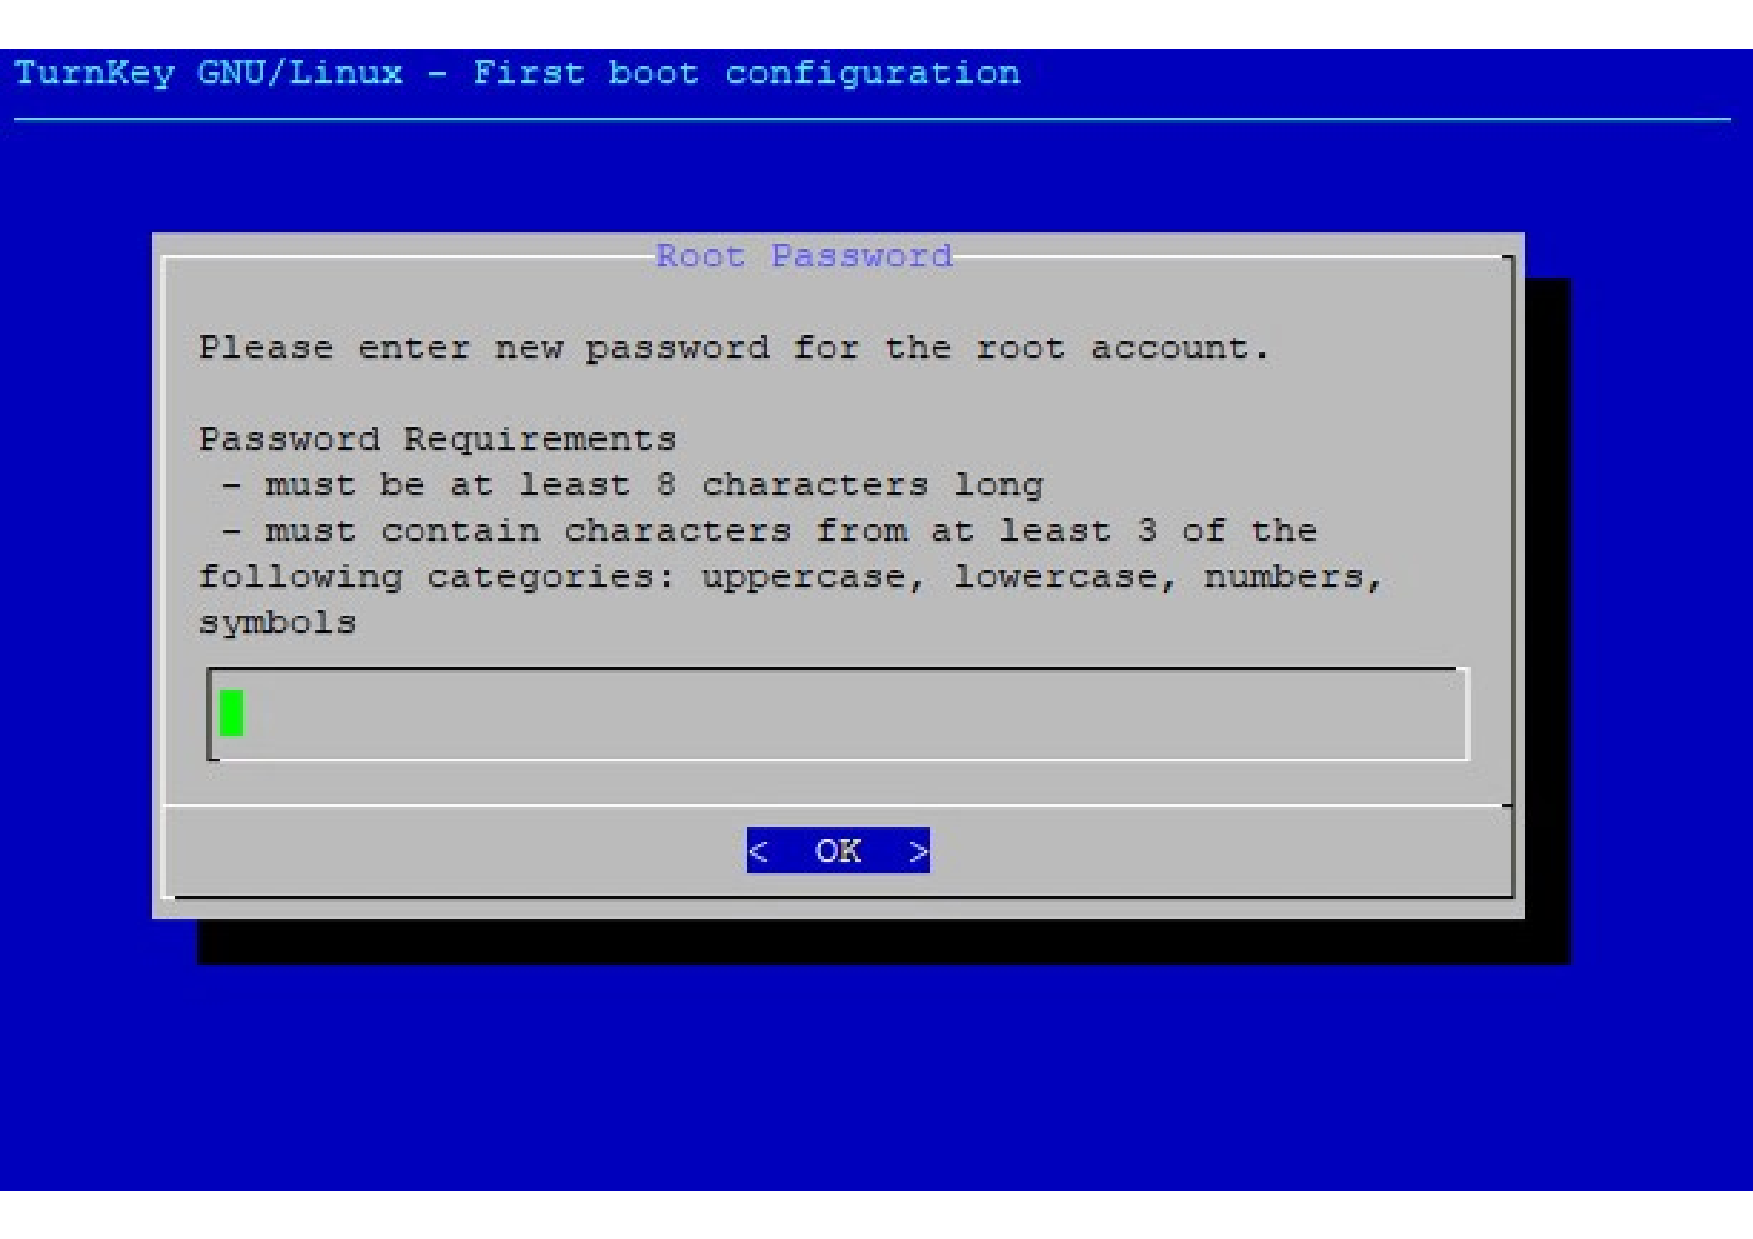
\includegraphics[width=1\linewidth]{chapters/images/root-pass.pdf}
    \caption{Interaktivní nastavení systému při prvním spuštění}
    \label{fig:inithooks-password}
\end{figure}

V případě spuštění bez grafického výstupu a uživatelských dat čeká systém na první přihlášení uživatele pomocí SSH s využitím přednastaveného klíče (přihlášení heslem
není k dispozici, neboť uživatel nenastavil heslo administrátora). Po prvním přihlášení dojde k automatickému spuštění zmíněného grafického průvodce.

\subsection{Výběr herního serveru}

K interaktivnímu výběru herního serveru dojde v případě, kdy uživatel nevybere požadovaný herní server pomocí uživatelského skriptu.
Do systému je tedy nutné přidat komponentu, která při prvním spuštění zobrazí seznam podporovaných herních serverů a umožní uživateli výběr.
K tomuto účelu bude využit mechanismus \mintinline{shell}{inithooks}, který umožní zobrazení komponenty při prvním spuštění systému.

Seznam podporovaných herních serverů závisí na zvoleném správci herních serverů. Je tedy nezbytné, aby komponenta uměla získat seznam těchto serverů
a zohlednila jej ve výběru.

\subsection{Automatická instalace a spuštění herního serveru}

Po výběru herního serveru je nutné tento server nainstalovat. Pro tento účet bude využit správce herních serverů, který dokáže stáhnout potřebné soubory
a provést instalaci. Je tedy třeba vytvořit komponentu, která provede přípravu na instalaci serveru a následně spustí správce.

\subsection{Nastavení herního serveru}

Mnohé herní servery vyžadují po instalaci dodatečnou konfiguraci. Může být nutné zvolit herní prostředí, jméno administrátora, jméno serveru a mnohé další parametry.
Je nezbytné implementovat mechanismus, který umožní uživateli provést toto nastavení interaktivně, případně automaticky.

Pokud uživatel spustí instanci systému bez předání potřebných dat, dojde k aktivaci mechanismu, který zajistí pozastavení veškeré činnosti systému do doby, než
se uživatel připojí k systému vzdáleně.


% \section{Operační systém}

% K tvorbě obrazu byl vybrán operační systém TurnKey GNU/Linux, který je primárně určený pro provoz aplikací v cloudovém prostředí.

% \section{Správce herních serverů}

